\chapter{Blockchain: il funzionamento e\\ i concetti principali}
\label{ch:blockchain}
% --- Inizio sezione 2 ---

Seguendo l’impostazione del lavoro presentata nell’introduzione è possibile individuare una prima nozione ricorrente, quella di “registro distribuito”. Negli ultimi anni l’estensione di Internet ha permesso di muovere i registri e generalmente parlando le informazioni e i dati, da un supporto fisico a un supporto digitale attraverso l’utilizzo delle basi di dati sparse in tutto il mondo. Tuttavia, la struttura attuale delle basi di dati e per certi aspetti l’architettura odierna di Internet, presentano dei problemi e degli svantaggi che, con l’andare del tempo non sono stati risolti in maniera definitiva. Basti pensare ai problemi relativi alla sicurezza, affidabilità e centralizzazione delle risorse memorizzate in rete.

Problematiche che, nella maggior parte dei contesti, possono essere ricondotte alla commercializzazione e centralizzazione delle risorse. Il punto chiave è che Internet allo stato attuale, Internet delle informazioni, si avvale di intermediari. Aziende come Google, Microsoft, Amazon e Facebook controllano una quantità enorme di informazioni e attività dei propri utenti. Un esempio del fenomeno può essere indotto dall’offerta di servizi di cloud computing (*aaS, anything as a service\footfullcite{wikiCloudComp}). Senza dubbio il vantaggio di questi servizi è che permettono agli utenti di usare risorse senza dover investire in un’infrastruttura propria e che sono offerti ad un costo relativamente basso. Si tratta pur sempre di intermediari verso quali è necessaria la fiducia che, con il passare del tempo, le corporazioni non sempre hanno dimostrato di gestire in maniera soddisfacente. Sono sorte preoccupazioni circa questioni importanti come la sicurezza, la censura e l'affidabilità di questi sistemi. Più in generale, i sintomi negativi della centralizzazione sono evidenti quando si parla dei problemi relativi alla privacy e all'uso inopportuno di dati privati, temi che ultimamente emergono di frequente. Ecco che avere opzioni, alternative in più a quelle già esistenti, può essere importante al fine di mitigare i rischi che possono essere causati da una situazione di monopolio e di concentrazione del potere nelle mani dei pochi.

La blockchain è un paradigma oppure semplificando, una tecnologia che potrebbe portare a una nuova evoluzione, un potenziale passaggio da un Internet delle informazioni all’Internet dei valori. Grazie all’uso della crittografia, del sistema di firme digitali, del networking peer-to-peer (P2P) e algoritmi di consenso, gli utenti possono effettuare transazioni che verranno mantenute in registri distribuiti, immutabili e permanenti senza bisogno di intermediari. In questo capitolo verranno descritti i concetti che formano l’insieme delle componenti di base delle blockchain.

\section{La struttura delle blockchain}

I concetti relativi alla struttura possono essere derivati dalla sua prima implementazione. Nel 2008 nasce Bitcoin, la prima applicazione su larga scala della tecnologia di seguito denominata blockchain. Fondata da Satoshi Nakamoto (autore o gruppo di autori anonimo), aveva come finalità la creazione di un sistema monetario digitale\footfullcite{Nakamoto_bitcoin:a}. Il sistema utilizza un registro pubblico, distribuito su tutti i nodi, contenente tutte le transazioni ordinate e valide, eseguite al suo interno fin dall’inizio della creazione del sistema stesso. Il concetto di sistema monetario digitale fu descritto già nel 1998 da Nick Szabo\footfullcite{SzaboDigCurr}, il quale aveva coniato il termine di certificati digitali al portatore (digital bearer certitifcate). Ancora prima, nel 1991, nell’articolo “How to Time-Stamp a Digital Document” di Stuart Haber e W. Scott Stornetta\footfullcite{Haber91howto} furono descritte quelle che sono le basi teoriche di un sistema decentralizzato. Questi documenti, rappresentano una fonte rilevante di approfondimento e sono importanti in quanto contengono l’espressione di concetti giudicati utili per la comunità ai fini di migliorare i sistemi digitali esistenti. Furono alla base della successiva ricerca sulla tecnologia, che ha condotto, a partire da Bitcoin, alla possibilità della sua implementazione concreta.

Al momento esistono oppure sono in via di sviluppo molte applicazioni e sistemi che utilizzano le blockchain, spesso la loro struttura costituisce un’estensione o un adattamento più sofisticato dei concetti iniziali a seconda delle funzionalità offerte. Questa è la motivazione per cui saranno presentati principalmente i concetti universali anche in funzione degli obiettivi finali per fornire un collegamento alle loro implementazioni e infine al caso concreto dell’archivio digitale.

\subsection{Distribuzione e decentralizzazione}

Prima di passare ai dettagli strutturali delle catene dei blocchi è importante distinguere tra due nozioni, quella di \emph{sistema distribuito} e \emph{decentralizzato}. Spesso, quando si parla di blockchain, i due termini sono usati come sinonimi. 

In realtà, dalle considerazioni precedenti è emerso che le blockchain implementano la tecnologia dei registri distribuiti collocando quest’ultima ad un livello di astrazione superiore. La DLT consiste nella condivisione di registri oppure, detto in un altro modo, base di dati a tutti i partecipanti del sistema. In questo caso i sistemi in questione sono le blockchain che, a loro volta vengono gestite da regole precise incapsulate nei sistemi di consenso (un argomento che verrà affrontato in dettaglio nel paragrafo 2.2). A questo punto è sufficiente dire che, grazie a questi sistemi di consenso, ogni nodo partecipante al sistema possiede una copia del registro e può interagire con esso effettuando modifiche che successivamente vengono aggregate con quelle di altri partecipanti. L’obiettivo è quello di mantenere una versione condivisa e sincronizzata del registro a tutti i partecipanti del sistema, in funzione delle regole di consenso della rete blockchain. Riassumendo si ha una completa distribuzione quando tutti i partecipanti sono in possesso di uno stesso registro.

Per quanto riguarda la nozione di decentralizzazione un approfondimento rilevante sulla questione è fornito in un articolo di Vitalik Buterin, uno dei fondatori del progetto Ethereum\footfullcite{Ethereum}. La sua idea è basata sulla suddivisione di un sistema e la sua centralizzazione o decentralizzazione lungo tre assi: quelli dell’architettura, della politica e della logica.
\\
\begin{figure}[H]
\centering
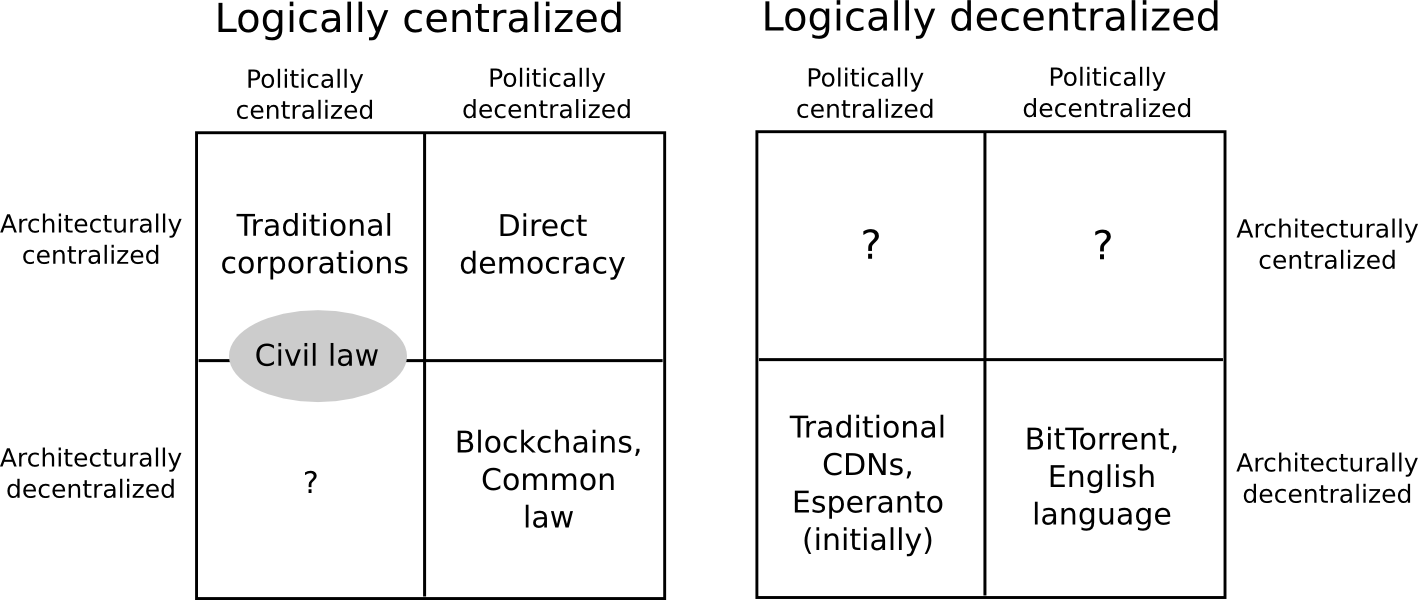
\includegraphics[width=1\textwidth]{immagini/meaning_decentralization.png}
\caption{Gli assi della decentralizzazione}
\label{fig:AssiDecentralizzazione}

\end{figure}

Secondo l’autore, come illustrato nella figura \ref{fig:AssiDecentralizzazione}, le blockchain sono architetturalmente e politicamente decentralizzate (nessuno esegue un controllo diretto su di esse e non c’è un punto centrale di guasto) ma logicamente centralizzate in quanto sono soggette a un preciso stato condiviso al momento dell'esecuzione del sistema che si comporta come un singolo computer\footfullcite{vitalButerinDecent}. Quest’ultimo aspetto, di nuovo, è fortemente legato ai protocolli di consenso che dipendono principalmente dalle varie tipologie di blockchain (un aspetto discusso nel paragrafo 2.4). La decentralizzazione riguarda maggiormente l’aspetto dei permessi dei partecipanti e la \emph{governance} sulla rete. La suddivisione descritta è valida per blockchain pubbliche (\emph{permissionless}) sulle quali si concentra questa tesi, in cui tutti i partecipanti hanno pari diritti di agire e modificare il registro condiviso. Per quanto riguarda la tipologia con permessi (\emph{permissioned}) la questione va riesaminata caso per caso, a seconda dell’implementazione concreta. 

Uno tra tanti esempi di quest’ultima tipologia è Ripple\footfullcite{rippleMain}, blockchain per trasferimento di fondi che nel suo sistema di validazione si avvale di un certo numero di attori imposti a priori perché ritenuti fidati dall'azienda. Questa politica comporta dei vantaggi dal punto di vista della scalabilità e della velocità di funzionamento a discapito della decentralizzazione dovuta alle forme di mediazione centralizzata. Attualmente, in questo specifico caso, con l’evoluzione della tecnologia blockchain questa strategia\footfullcite{rippleStrategy} viene rivista a favore di una maggiore decentralizzazione. Gli aspetti pro e contro l’adozione di sistemi più o meno decentralizzati sono discussi nel paragrafo (2.3.3).

Finalmente, distinte queste due nozioni è possibile arrivare alla seguente conclusione: il paradigma blockchain è distribuito (i partecipanti sono in possesso del registro replicato) mentre a livello inferiore, delle implementazioni, le blockchain possono essere più o meno decentralizzate (o centralizzate) a seconda degli obiettivi e delle funzionalità che intendono raggiungere.

\subsection{Transazioni e concatenazione di blocchi}

Le blockchain utilizzano, letteralmente, una struttura pensata come una catena di blocchi. Ciascun blocco contiene al suo interno una lista di transazioni immutabili a loro volta contrassegnate da delle proprietà. Nelle attuali implementazioni le proprietà fondamentali sono:

\begin{itemize}
\item indirizzo mittente (input) 
\item indirizzo destinatario (output)
\item ammontare di valuta o token contenuto nella transazione
\item marcatura temporale (timestamp)
\end{itemize}

In una rete di consenso decentralizzato vengono man mano inseriti dei blocchi contenenti al loro interno un certo numero di transazioni. A livello universale, di rete, questa catena viene gestita dagli algoritmi di consenso come ad esempio: Proof of Work e Proof of Stake (descritti nel paragrafo 2.1.4) appendendo i blocchi giudicati validi dopo l'ultimo blocco valido della catena in modo da creare un registro di operazioni ordinato cronologicamente. Una volta stabilita la legittimità di un blocco e la sua appartenenza alla catena valida più lunga, l’intera struttura viene aggiornata propagando (analogamente a come avviene nel modello peer-to-peer) i nuovi elementi a tutti i partecipanti del sistema. Lo stato del registro, a questo punto, non è più soggetto a modifiche, diventa permanente e immutabile. Successivamente il procedimento riparte ricorsivamente, come descritto, ampliando la catena con le nuove operazioni.

Il primo blocco\footfullcite{genesisBitc} \smallskip \footfullcite{genesisEth} (programmato manualmente cioè \emph{hardcoded}), originario di tutta la catena è chiamato \emph{genesi}. È un blocco speciale perché non è preceduto da altri blocchi, in esso vengono programmate le proprietà dei blocchi futuri. Le specifiche cambiano a seconda dell’implementazione. Generalmente si tende a definire proprietà come la grandezza del blocco, la difficoltà di appendere nuovi blocchi e la ricompensa per la creazione (validazione) di nuovi blocchi nel sistema. 
Seguendo questo ragionamento, il seguente è un esempio valido di un blocco generico che eredita le sue proprietà dal blocco genesi.
Di seguito, insieme alle spiegazioni di alcuni concetti si forniscono pezzi di codice (code snippets) per illustrare la relativa struttura semplificata (il codice rispetta la sintassi Javascript ECMAScript 2015\footfullcite{jsDocs}). 

\begin{lstlisting}[caption={Esempio di struttura di un blocco},language=JavaScript]
class block {
    constructor(timestamp, transactions, prevHash ='') {
        this.timestamp = timestamp;
        this.transactions = transactions;
        this.prevHash = prevHash;
        this.hash = this.calculateHash();
        this.nonce = 0;
    }
\end{lstlisting}

Ancora una volta, tra le proprietà importanti per il protocollo, si possono distinguere: la marcatura temporale che corrisponde alla data di creazione del blocco, la lista di transazioni incluse nel blocco, e la connessione tra i blocchi ovvero il "legame" calcolato tramite la funzione hash tra il blocco successivo e il precedente.

Combinando insieme i blocchi si otterrà la seguente panoramica della struttura:

\begin{figure}[H]
\centering
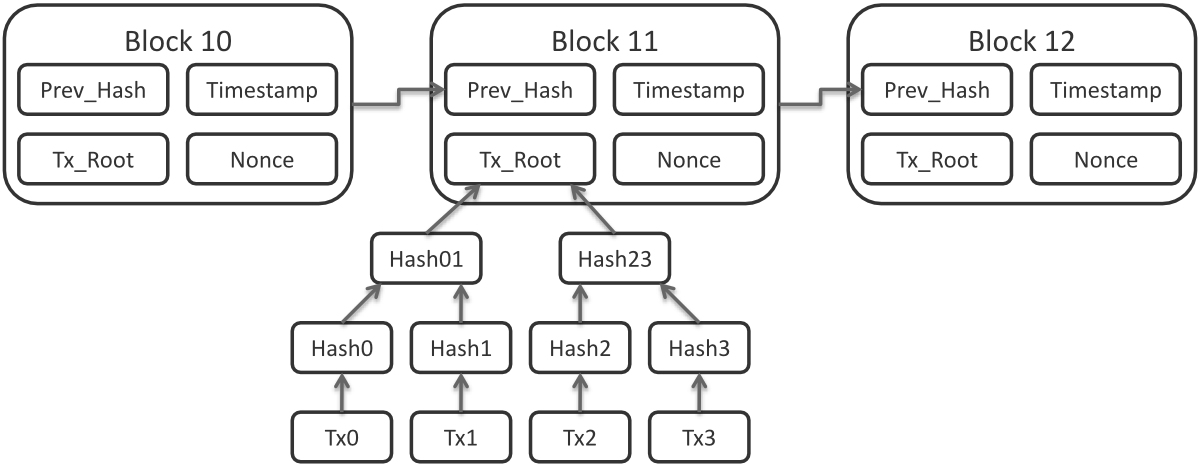
\includegraphics[width=1\textwidth]{immagini/bitcoinblocks.png}
\caption{Struttura semplificata di una catena di blocchi}
\label{fig:ConcettoStrutturaBlocchi}

\end{figure}

Tenendo in mente che l'impostazione di un blocco può contenere un numero di proprietà variabile (a seconda dell'implementazione), è possibile generalizzare una struttura come quella illustrata nella figura 2.2. Nelle sezioni successive saranno analizzati gli elementi costituenti dei blocchi e le procedure che ne determinano il funzionamento.

\subsection{Funzioni di hash}

Ogni blocco è legato al blocco precedente tramite una funzione hash calcolata in base alle proprietà del blocco. Una funzione hash è una funzione matematica unidirezionale che accetta un input di lunghezza arbitraria e ne produce un output di lunghezza prefissata.

È una delle componenti base di una struttura formata da sequenze di blocchi che a sua volta è paragonabile alla struttura di una lista concatenata (\emph{linked list}) tramite puntatori. In entrambi i casi la struttura permette di identificare in maniera univoca la relazione precedente e successivo che intercorre tra due blocchi. Dunque, data la definizione della funzione hash, il suo risultato dipende dalle proprietà di ciascun blocco.

Senza entrare troppo in dettaglio, questo implica un insieme di proprietà "grande" su quale vengono calcolate le funzioni hash con la caratteristica che, anche una minima variazione di ciascun componente del dominio della funzione, molto probabilmente farà cambiare radicalmente il risultato calcolato.
Nel seguente esempio si calcola la funzione hash applicando l'algoritmo SHA256 (Secure Hashing Algorithm\footfullcite{sha2Wiki}), utilizzata nelle blockchain (per esempio Bitcoin) per due input apparentemente simili: 

\begin{lstlisting}[caption={Esempio di calcolo della funzione hash SHA256},language=JavaScript]
//Input 1: ciao Tizio
>> SHA256("ciao Tizio")
//Output 1: 
>> 875647588afa538ef3645bcdf413497af42461ea09e8f79df69b7a95c229d2a5
//Input 2: ciao tizio
>> SHA256("ciao tizio")
//Output 2: 
>> 961e89e74136c7094097f1a625b596f5df27cc6a71e0031bacf609e09feb2634
\end{lstlisting}

Si vede che anche la più piccola variazione in input produce (con probabilità estremamente alta) un output (righe 4,8) molto diverso.\footfullcite{hashExample}
Continuando con questo ragionamento, i blocchi sono formati da un insieme di proprietà che messe insieme produrranno una hash unica. Considerando il seguente esempio di calcolo della proprietà prevHash di un blocco:

\begin{lstlisting}[caption={Esempio di calcolo della funzione hash in base alle proprietà del blocco},language=JavaScript]
>> SHA256(prevHash+timestamp+transactions+nonce)
\end{lstlisting}

È chiaro, a questo punto cosa si intende per quello che all'inizio di questa sezione veniva chiamato: "un'insieme di proprietà grande". Con più precisione, in qualsiasi blocco, il dominio della funzione hash è formato da (sempre in riferimento all'esempio della figura \ref{fig:ConcettoStrutturaBlocchi}): marcatura temporale, il risultato delle continue applicazioni di hashing proprie di ciascuna transazione (tx root), il numero pseudocasuale (nonce) e il risultato della funzione hash del blocco precedente. In breve, vengono messe insieme tutte queste informazioni (paragonabile a una “polpetta” fatta da un composto di altri “elementi”) contenute nel blocco per produrre un unico hash. Questo non è l'unico caso in cui l'utilizzo di questa funzione è fondamentale, lo hashing delle transazioni è stato menzionato per introdurre un livello di dettaglio ulteriore. Nella prossima sezione, a proposito delle continue applicazioni delle funzioni hash, verrà introdotta la struttura, Merkle Tree (albero di hash).

Infine, disponendo della vista d'insieme dell'algoritmo di hashing, ne deriva la sicurezza dell'intero sistema. Supponendo uno o più attacchi con l'obbiettivo di alterare il contenuto dei blocchi il malintenzionato dovrà ricalcolare tutti gli hash dei blocchi successivi per validare l'intera catena e dovrà farlo prima che un nuovo blocco arrivi validato dal sistema di consenso. In questo caso la priorità è della catena più lunga quindi l’eventuale attaccante sarà costretto a ricalcolare gli hash della nuova catena dall’inizio. Quello della sicurezza è un concetto che dipende dal sistema di consenso implementato e verrà discusso in seguito con maggior dettaglio.

\subsection{Merkle Trees}

Gli alberi di hash sono una struttura dati utilizzata nelle blockchain. È una delle componenti del blocco le cui proprietà fondamentali si sono ipotizzate negli esempi delle sezioni precedenti. In particolare, nella figura \ref{fig:ConcettoStrutturaBlocchi} è presente la radice (tx root) di un merkle tree. La radice è il risultato di applicazioni continue di operazioni hash a partire dal livello con cardinalità più alta (ipotizzando che la cardinalità della radice sia minore di quella dei suoi figli). Il motivo per cui viene usata questa struttura è da ricondurre all'efficienza degli alberi di hash, nel memorizzare, nel caso delle blockchain, le transazioni. 


\begin{figure}[H]
\centering
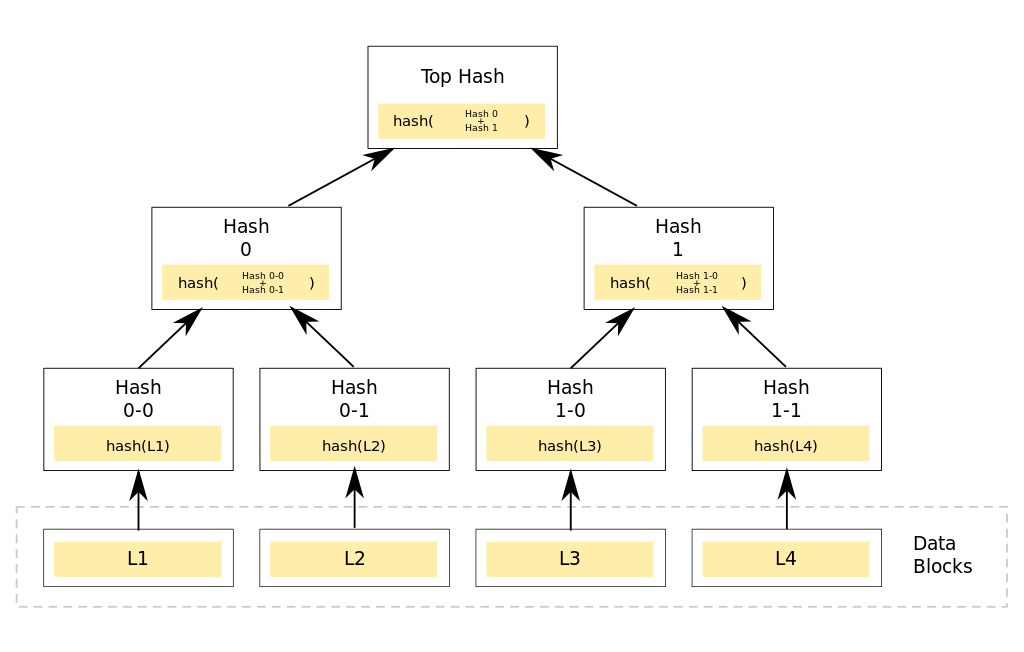
\includegraphics[width=1\textwidth]{immagini/hash_Trees.png}
\caption{Struttura di Merkle Tree}
\label{fig:MerkleTreeStruttura}

\end{figure}

La figura \ref{fig:MerkleTreeStruttura} rappresenta un albero di hash binario che può essere generalizzato per visualizzare il procedimento di hashing di un numero arbitrario di transazioni (limitate nella definizione del blocco). Nell'esempio a partire dal basso (o a livello di cardinalità più alto, nelle foglie) si trova contenuto l'insieme delle singole transazioni (L1-L4).

Il primo passo consiste nell’eseguire l'algoritmo di hashing sulle singole transazioni. L'output di queste operazioni viene successivamente accoppiato con il risultato dell'elemento (nodo) adiacente e su di essi viene di nuovo eseguito l'algoritmo di hashing. Il procedimento è ripetuto ricorsivamente fino a giungere alla radice, risultato di continue applicazioni di hashing nell'insieme di nodi, i quali si trovano a sinistra e a destra rispetto alla radice. Dunque, ogni nodo è l'hash dei suoi figli\footfullcite{ethWhitepaper}. 

Una delle proprietà delle funzioni crittografiche di hash (come SHA-2) consiste, dal punto di vista computazionale nell'essere veloce da calcolare su qualunque tipo di dato. Inoltre la peculiarità di questa struttura è che appendere nuove foglie, equivalenti a nuove transazioni che vengono man mano aggiunte all’albero, non comporta la ricomputazione dell’intera struttura, ma solo del percorso che porta direttamente alla radice.

Il vantaggio dal punto di vista dell'efficienza dei merkle trees deriva proprio da questa impostazione della struttura gerarchica definita dagli elementi sottostanti. Si tratta dell'efficienza in termini di tempo e di spazio necessario per memorizzare la struttura. La finalità di Merkle Trees deriva dalla frammentazione dei dati al suo interno e la loro composizione nella radice, sotto un unico identificatore hash. In questo modo, per assicurare l'integrità delle transazioni del blocco, sarà sufficiente verificare la radice della struttura (tx root). Questo è possibile perché la propagazione con la messa insieme di funzioni hash avviene sequenzialmente dalle foglie alla radice.

A livello della blockchain questo apre diverse possibilità di verifica dell'integrità delle singole transazioni e la possibilità di ridurre lo spazio e il tempo necessario per sincronizzare la catena dei blocchi aggiornata all'ultima versione valida. Ad esempio, per un membro della rete che non intende effettuare operazioni su singole transazioni dei blocchi sarà sufficiente verificare solo gli hash contenuti nell'intestazione (header) dei blocchi per avere una prova sufficiente della correttezza dei dati all'interno della struttura. Questa caratteristica di Merkle Tree prende il nome di \emph{Merkle proof} (prova di correttezza) e vale per qualsiasi elemento della struttura. Dunque supponendo che questa struttura venga usata per memorizzare una grande quantità di dati, controllare che un frammento di questi dati sia consistente, verrà controllato il percorso che collega il dato elemento alla radice. Questo equivale a rieseguire calcoli delle funzioni hash su specifici frammenti di dati e controllare i risultati con quelli già calcolati da altri nodi della rete per confermare la loro correttezza e quindi la validità per la blockchain.

\section{Il sistema di consenso} %  Inizio sezione 2.2

Una volta definito il funzionamento concettuale di una rete blockchain sorge il dubbio come questo proliferare di operazioni, di calcolo delle funzioni hash, dell'addizione dei nuovi blocchi alla catena e più in generale l'insieme delle operazioni di gestione dell'intera struttura siano possibili in un ecosistema decentralizzato. 

Innanzitutto, le blockchain decentralizzate operano in maniera incentivata. La disintermediazione è garantita dagli algoritmi di consenso che stabiliscono le regole di funzionamento della rete. Nel caso delle blockchain pubbliche si tratta di una rete dove tutti i partecipanti sono alla pari, possono proporre nuove transazioni e tutti insieme devono mettersi d'accordo su quali transazioni effettivamente aggiungere al registro comune. Si vede delineato un contesto in cui è presente un insieme di partecipanti, ciascuno avente i propri interessi ma nonostante obiettivi spesso contrapposti l'intero sistema deve giungere a un consenso. Tipicamente l'incentivazione consiste in una ricompensa, una quantità di valuta o token, spettante al nodo o ai nodi a cui viene dato il potere di appendere un blocco alla catena. L’approfondimento di questo aspetto economico è strettamente legato al tipo di algoritmo di consenso implementato, alcuni dei quali (ad esempio, Proof of Work e Proof of Stake), verranno discussi più avanti in questa sezione.

\subsection{Il problema dei generali bizantini}

Dal punto di vista teorico, la difficoltà di consenso può essere ricondotta al problema dei generali bizantini\footfullcite{byzantine-generals-problem}. In una delle possibili formulazioni del problema si suppone che una città venga assediata da molti eserciti con a capo un generale. Per ottenere la vittoria tutti gli eserciti devono raggiungere un consenso e attaccare simultaneamente altrimenti, se non attaccano in numero sufficiente, verranno sconfitti. Il generale manda l’ordine attraverso dei messaggeri ai comandanti degli eserciti che, a loro volta possono mentire scegliendo arbitrariamente di passare ordini diversi e di tradire il generale e gli altri comandanti.

Dunque è una situazione che si porta bene a essere visualizzata all'interno delle blockchain (propriamente decentralizzate). In riferimento al problema sopra esposto si fa a meno del generale che manda degli ordini ai suoi sottoposti. Nella pratica, si tratta di una rete dove tutti i partecipanti possono proporre nuove transazioni e tutti insieme devono mettersi d'accordo su quali transazioni effettivamente aggiungere al registro comune in mancanza di un nodo generalmente definibile come detentore della verità (\emph{holder of truth}). Il punto chiave è che tutti i componenti del sistema devono prendere la stessa decisione (e non necessariamente la decisione ritenuta “giusta”) su un piano di parità, cioè senza l’esistenza di un’entità “fidata” che possa provarne l’autenticità. Tutto questo in un contesto di presenza di potenziali nodi "traditori" che minacciano l'integrità della rete. In riferimento a questi nodi viene sollevata la questione della fiducia che deriva dall'implementazione delle regole di consenso. La struttura delle blockchain (l’aggiunta di nuovi blocchi quindi la validazione delle transazioni) è controllata da queste regole le cui implementazioni implicano anche l'esistenza di un limite che se superato permette di approvare operazioni illecite e potenzialmente corrompere l'intera rete. Questo limite, a seconda dell’algoritmo utilizzato, riguarda la potenza computazionale necessaria per superare il controllo di validazione e il numero di nodi che decidono di mettersi d'accordo per approvare operazioni al di fuori dalle regole del sistema. Un esempio concreto, nella rete Bitcoin, la potenza computazionale necessaria per compromettere la rete è maggiore del 50\% totale della capacità computazionale dell’intera rete\footfullcite{btcAttacchi1}. Questa soglia cresce man mano che i potenziali attaccanti vorrebbero modificare le transazioni contenute nei blocchi precedenti\footfullcite{btcAttacchi2}.

In questo modo, grazie al consenso distribuito, le blockchain riescono a rimediare al problema dei generali bizantini (BFT, \emph{Byzantine Fault Tolerance}) in un ecosistema distribuito. Questo, come già accennato, è garantito dagli algoritmi di consenso implementati nella rete, di cui i principali Proof of Work e Proof of Stake. Nell’insieme BFT contribuisce alla sicurezza della rete e previene il fenomeno della doppia spesa \footfullcite{btcSicurezza}.


\subsection{Proof of Work}

Proof of Work, cronologicamente, è il primo sistema di consenso usato nelle blockchain implementato per la prima volta da Bitcoin con lo scopo di raggiungere un consenso tra in nodi presenti sulla rete circa lo stato dell’intero sistema. La sua finalità consiste nella gestione e nell'aggiornamento della catena dei blocchi con i relativi elementi in modo che i tutti i partecipanti siano “in linea” con la versione della catena valida cioè con la sequenza dei blocchi più lunga. Il legame tra i blocchi, una volta validato dall'algoritmo comporta la creazione di una struttura di contenuti immutabile comprendente tutta la storia delle operazioni intercorse fin dalla creazione del blocco genesi.

\begin{figure}[H]
\centering
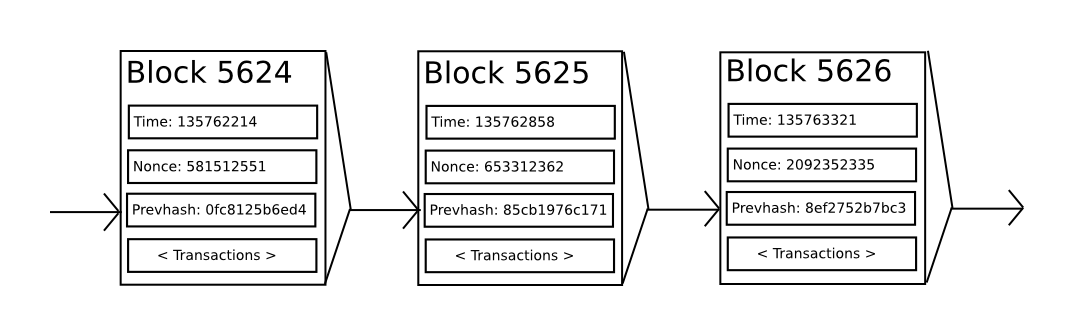
\includegraphics[width=1\textwidth]{immagini/mining_pow.png}
\caption{Mining: Proof of Work}
\label{fig:ProofOfWork}
\end{figure}

Nella figura \ref{fig:ProofOfWork} è illustrato il processo di creazione di nuovi blocchi collegati mediante il riferimento all'indirizzo hash del blocco precedente. Da notare: il tempo di creazione del blocco strettamente crescente dovuto al funzionamento di Proof of Work che sequenzialmente, a intervalli regolari, permette l'inserimento nella rete di un blocco valido. Messe insieme: la quantità di computazione richiesta e la creazione di blocchi a intervalli regolari diventa possibile rimediare ai problemi di congestione della rete, dovuti alla creazione di una quantità di transazioni troppo grande da essere processata in tempi ragionevoli (così come avviene negli attacchi di tipo DDOS).

Senza un punto centrale di calcolo il procedimento di validazione è incentivato per permettere il funzionamento affidabile e costante in un sistema distribuito. Nel caso di Proof of Work, i membri della rete blockchain possono partecipare a una competizione con l’obbiettivo di appendere un blocco alla catena e ricevere in cambio una ricompensa. Si tratta di dimostrare di aver compiuto una quantità di calcoli computazionali per mezzo di cosiddetti “puzzle crittografici”. Queste dimostrazioni possono, ad esempio sfruttare la caratteristica della distribuzione uniforme delle funzioni crittografiche di hash per cui il calcolo di una funzione hash comporta la generazione di un risultato, il quale, come dimostrazione, dovrebbe appartenere a un insieme ristretto del dominio dei possibili risultati. Relativamente alla crescita e all'incremento della potenza computazionale dei calcolatori è consigliabile che questa dimostrazione sia controllata da una difficoltà variabile, anch’essa crescente in relazione all’aumento di \emph{hashrate} (la frequenza di calcolo della funzione hash). Ad esempio una dimostrazione Proof of Work potrebbe richiedere che un numero arbitrario di cifre del risultato generato dalla funzione hash sia uguale a zero. Successivamente l’incremento della difficoltà consiste nell’incremento di questo numero di cifre. Di conseguenza, l’aumento di \emph{hashrate} è direttamente proporzionale alla probabilità di venire selezionati come creatori del nuovo blocco e quindi ricevere la ricompensa.

Per ribadire quanto è stato appena detto si suppone che la dimostrazione richieda che le prime tre cifre della funzione hash calcolata siano pari a zero.
A questo scopo si riprende l'esempio del codice 2.3: Esempio di calcolo della funzione hash, in base alle proprietà del blocco. 
\\
\begin{lstlisting}[caption={Esempio di calcolo della funzione hash in base alle proprietà del blocco},language=JavaScript]
function calculateHash(difficulty) {
    nonce = nonce + 1;
    return SHA256(prevHash+timestamp+transactions+nonce);
}
...
//Output per nonce = 10:
3747cd1b31b876bda0bf8540ad4eeb115239c2d69835a74cc5835d9d3b3f3b27
//Output per nonce = 11:
aac295677f4761d411bc4fdb2953ac3ce2a2b8202207928a8db1cdac45aa8885
...
//Output per nonce = 10390:
0000b280f48a4640ea18e2b6ee999fc60bfc85b690e990c0bdc4f9ae2b1e13c6

\end{lstlisting}

A ogni iterazione viene generato il risultato della riga 3 e successivamente confrontato con la difficoltà che in questo esempio supponiamo sia pari a quattro zeri iniziali. Concretamente il numero di questi tentativi fatti in un secondo prende il nome di \emph{hashrate}. Se il risultato non soddisfa la dimostrazione allora viene incrementata di uno la proprietà nonce, numero arbitrario che può essere usato una volta sola. Siccome anche una minima variazione in input probabilmente farà cambiare radicalmente il risultato, ad un certo punto verrà generato un risultato che soddisfa i requisiti prestabiliti nella proprietà della difficoltà. Nella simulazione effettuata utilizzando una versione estesa di calculateHash l'output della riga 12 è stato trovato, dopo pochi secondi, al 10.390 tentativo. Per ottenere il risultato con cinque cifre iniziali uguali a zero ci è voluto circa un minuto e 426.203 tentativi.
\\

\begin{figure}[H]
\centering
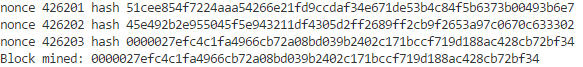
\includegraphics[width=1\textwidth]{immagini/miningOutput.png}
\caption{Mining: Risultato simulazione}
\label{fig:SimulazionePoW}
\end{figure}

In conseguenza, nelle applicazioni reali, succede che questa dimostrazione di calcoli computazionali porta con sé il consumo di una quantità enorme di energia elettrica. Evidentemente questo può essere considerato come uno spreco con un impatto negativo nei vari contesti generali come l’ambiente, il favoreggiamento di utenti con infrastruttura più efficiente (ad esempio, \emph{mining pools\footnote{Le mining pool ragruppano utenti chiamati miner che, decidono di condividere la propria potenza computazionale per collaborare al processo di creazione dei blocchi. In questo modo la ricompensa sarà equamente distribuita a tutti i partecipanti di un certo gruppo (pool) di miner}}) ecc.
Si ipotizza che, attualmente, il consumo di energia annuo di Bitcoin sia di circa 2.55 GW, paragonabile al consumo annuo dei paesi come l’Irlanda (circa 3.1 GW) e in questa forma è destinato a crescere\footfullcite{btcEnergy}.

\subsection{Proof of Stake}

Per contrastare le conseguenze negative derivanti dall’utilizzo di Proof of Work sono stati sviluppati oppure sono in produzione altri sistemi di consenso. Il perno della costruzione di questi sistemi riguarda proprio la fase di dimostrazione che contribuisce alla sicurezza e integrità della rete, così come descritta in Proof of Work. Tra i sistemi più promettenti è stato definito Proof of Stake, il quale riesce a risolvere il problema di consumo incrementale di energia dovuto alla quantità di calcoli computazionali.

Questo algoritmo si basa su un processo di elezione. All’interno della rete blockchain, gli utenti possono scegliere di entrare a far parte di un gruppo di utenti, aperto a tutti, chiamati validatori. Per poter partecipare a questo processo è sufficiente depositare una quantità di valuta o token che verrà conservata nella rete come deposito (\emph{stake}). Analogamente a Proof of Work a ogni partecipante, nel caso di Proof of Stake chiamato validatore al posto di miner, viene concesso il potere di appendere un blocco alla blockchain ricevendo in cambio una ricompensa (di solito una parte delle commissioni incluse nell’insieme delle transazioni del blocco). Il nodo validatore può essere scelto seguendo un processo di selezione casuale e tenendo conto della quantità del deposito messo a disposizione. I vantaggi di questo approccio sono evidenti dal punto di vista dell’efficienza computazionale. Inoltre, con la crescita della rete e la quantità di criptovaluta circolante al suo interno diventa teoricamente impraticabile effettuare un attacco della maggioranza\footfullcite{btcAttacchi1} che, tra le altre cose può essere ulteriormente contrastato introducendo una certa variabile di casualità al processo di selezione del validatore. La scelta di particolari soluzioni dipende dalle diverse implementazioni dell'algoritmo, relativamente a Proof of Stake è opportuno menzionare che il deposito di validatori disonesti, cioè di coloro che cercano di approvare transazioni fraudolente, non sarà restituito e in tal caso questi perderebbero dei soldi. Lo stesso deposito sarà mantenuto dalla rete per un certo periodo di tempo necessario per provare che non siano state accettate transazioni fraudolente da parte del validatore.

% Fine sezione 2.2

\section{Funzionamento dell'ecosistema blockchain} % Inizio sezione 2.3

L’insieme dei concetti presentati, contribuisce al funzionamento delle blockchain in un contesto distribuito. In questo capitolo sarà approfondito il legame tra queste componenti per capire meglio il funzionamento dell’intera rete. In molti casi, l’adozione delle blockchain porta con sé vantaggi, ma anche ripercussioni circa questioni come la scalabilità e i costi di funzionamento.

Saranno introdotte alcune ulteriori caratteristiche della tecnologia che derivano dai concetti presentati nel primo capitolo e che, per motivi di chiarezza dell’esposizione non erano adatte ad essere inserite nelle loro parti introduttive. In molti casi le diverse componenti collaborano alla creazione di caratteristiche e di soluzioni e pertanto è lecito parlarne solo dopo che sono state introdotte nel loro insieme.

\subsection{Transazioni e prevenzione della doppia spesa}

Tra le componenti fondamentali delle blockchain un ruolo di primo piano spetta alle transazioni. Dopo una prima definizione nel capitolo 2.1 in relazione alla struttura della rete, queste necessitano di ulteriori approfondimenti.

I primi due elementi essenziali per poter effettuare una transazione sono: l’indirizzo mittente e destinatario. Questi indirizzi corrispondono agli account degli utenti che effettuano e ricevono le transazioni. Così come avviene nelle applicazioni web tradizionali, gli account vengono identificati da un username e una password, nelle blockchain vengono semplicemente usati indirizzi (\emph{address}) univoci. Questo non solo è sufficiente ai fini dell’autenticazione, ma contribuisce alla sicurezza grazie all’uso della crittografia asimmetrica\footfullcite{wikiAsymEncrypt} e al sistema di firme digitali\footfullcite{wikiDigSign}. Questa estensione delle transazioni si presta bene ad essere visualizzata attraverso un semplice esempio di trasferimento di token da un indirizzo ad un altro.
\\

\begin{figure}[H]
\centering
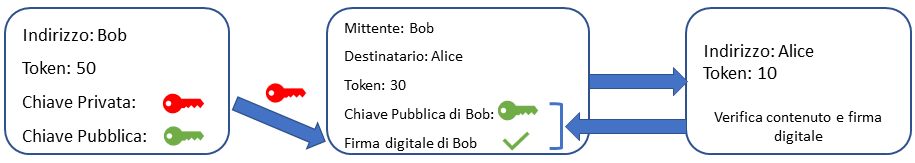
\includegraphics[width=1\textwidth]{immagini/transazioneFinal.png}
\caption{Transazione: Trasferimento Token}
\label{fig:TransazioneToken}
\end{figure}

Nella transazione, in figura \ref{fig:TransazioneToken}, vengono inviati 20 token (o qualunque criptovaluta implementata nella blockchain) verso un altro utente della rete. L’uso della crittografia asimmetrica permette di condividere la propria chiave pubblica all’intera rete in modo da poter essere identificati, in questo caso, come mittente della transazione. Dall’altra parte la chiave privata (segreta) corrisponde per certe caratteristiche alle tradizionali password in quanto prova il possesso della chiave pubblica e pertanto consente di identificare in maniera sicura l’utente ma in più permette anche di firmare le transazioni. Una transazione firmata, cioè dotata di firma digitale, costruita combinando la chiave privata del mittente e il contenuto della transazione, assicura l’integrità e la provenienza della transazione. Un algoritmo verificherà la firma digitale determinando se il contenuto corrisponde a quello originale e quindi se non è stato modificato.
\\

\begin{figure}[H]
\centering
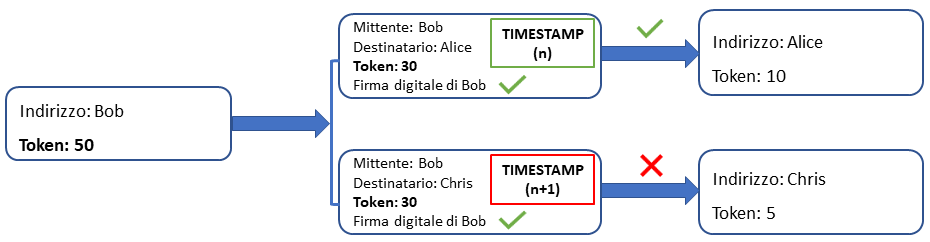
\includegraphics[width=1\textwidth]{immagini/doubleSpend.png}
\caption{Transazione: Doppia Spesa}
\label{fig:TransazioneDoppiaSpesa}
\end{figure}

Un altro problema fondamentale circa le transazioni è il problema della doppia spesa illustrato nella figura \ref{fig:TransazioneDoppiaSpesa}. Consiste essenzialmente nell’abilità di spendere più di una volta la stessa quantità di valuta. La prima applicazione della blockchain aveva come scopo la creazione di un sistema monetario digitale dunque era fondamentale risolvere la questione. Effettivamente, combinando le caratteristiche delle blockchain, il sistema di consenso e la crittografia, il problema della doppia spesa può essere risolto in un ecosistema decentralizzato\footfullcite{btcSicurezza}. 

In dettaglio le transazioni contengono una propria marcatura temporale e durante il loro processo di validazione seguono il criterio della sequenzialità. Il tutto avviene in un contesto trasparente con a disposizione tutta la storia delle transazioni avvenute nel sistema (equivalente a una base di dati dotata di storia completa). In questo modo il contenuto delle transazioni è interamente tracciabile e pertanto può essere esplicitamente validata la loro effettiva disponibilità, in questo caso, di token. Seguendo questo ragionamento in realtà non sarebbe necessario tenere un bilancio esplicito di token totali, ma analizzando lo storico complessivo dei trasferimenti di valori specifici, è possibile risalire all’importo in questione da cui deriva la trasparenza della rete blockchain.

\subsection{Teoria dei giochi e governabilità}

Una nozione importante per il funzionamento del paradigma blockchain è relativa al sistema di consenso incentivato. Riprendendo il principio delle blockchain pubbliche ogni utente dovrebbe, in qualunque momento, essere in grado di partecipare ed effettuare modifiche al registro comune affidandosi alle regole della rete che garantiscono la terminazione delle operazioni effettuate. Le blockchain, così come tutti gli altri servizi web, devono essere in grado di offrire un servizio consistente producendo risultati deterministici con la peculiarità del contesto distribuito e decentralizzato.

Nell’assenza di un’entità centrale l’obiettivo viene raggiunto applicando un sistema di ricompense che segue i principi della teoria dei giochi\footfullcite{wikiGameTheory}. Un modello ragionevole, dal punto di vista economico, cerca di mantenere un equilibrio tra ricompense previste per utenti che seguono le regole e punizioni per chi le trasgredisce. In precedenza (nel capitolo 2.2) si è visto che a intervalli di tempo regolari viene avviata una competizione, al vincitore della quale spetta il potere di appendere un blocco alla catena e ricevere la ricompensa prevista. Detto questo i dettagli sono strettamente legati alle singole implementazioni della tecnologia. Generalmente si cerca di promuovere la cooperazione a beneficio della rete e quindi di tutti gli utenti. L'obiettivo finale è quello di costruire la fiducia in una rete non supervisionata, creando condizioni in cui i procedimenti di verifica o validazione siano ricompensati e quindi benefici per l’intero sistema.

Un contesto decentralizzato implica anche l’adozione di regole di \emph{governance} precise. Queste regole e procedure riguardano proprio la gestione e il controllo di questo fenomeno collettivo, messo in pratica, attraverso una rete decentralizzata. La governance riguarda tradizionalmente: la fiducia nelle istituzioni, enti centralizzati, governi ecc. Per l’oggetto di questa tesi la governance si fonda sulle tecnologie di regolamentazione basate sulla trasparenza, disponibilità di dati immutabili e permanenti, sulla esecuzione automatica di contratti (smart contracts di cui si parlerà nel capitolo 3.2) e su una gestione comunitaria dell’intera rete.

Secondo gli analisti della STOA (Science and Technology Options Assessment), gruppo di ricerca del parlamento europeo, le blockchain potrebbero portare alla diffusione di \emph{organizzazioni autonome decentralizzate} (\emph{DAO}) governate dalla collettività. I potenziali sviluppi di un nuovo sistema di governance possono favorire la nascita di sistemi organizzati, non più gerarchicamente attraverso il controllo dall’alto verso il basso, ma più democratici ed efficienti, dotati di utilità sociale che rispecchia direttamente i valori perseguiti dalla comunità\footfullcite{eu-parl-paper}.

\subsection{Trilemma scalability}

L'adozione di tutti questi concetti potenzialmente rivoluzionari porta con sé anche dei compromessi. Per poter presentare l’estensione del problema un esempio significante riguarda la velocità del funzionamento. In relazione ai sistemi in uso come il protocollo finanziario \emph{Visa}, le blockchain pubbliche sono molto più lente. Il sistema Visa, in media, è in grado di processare circa 1.700 transazioni al secondo (con potenziali capacità di scalabilità di oltre 24.000 transazioni al secondo\footfullcite{visaThroughput}), mentre allo stato dell’arte attuale, il throughput (inteso come capacità di processare le operazioni) per le blockchain più popolari Bitcoin ed Ethereum è pari rispettivamente a circa 7 transazioni al secondo e 15 transazioni al secondo nel caso di Ethereum. Si può notare che le transazioni Visa sono puramente finanziarie mentre il vantaggio delle blockchain deriva dalla possibilità di poter processare qualunque tipo di operazione di scambio. Tuttavia il problema persiste (e non è correlato alla tipologia delle transazioni), ed è difficilmente accettabile che, al crescere della rete, gli utenti siano disposti ad aspettare tempi sempre più lunghi dovuti al processo di validazione (creazione di nuovi blocchi di transazioni controllata dal sistema di consenso). Un discorso simile può essere fatto per la scalabilità in termini di spazio, i registri distribuiti dotati di storia completa devono essere sincronizzati per potervi partecipare in maniera sicura. Questo comporta uno spazio in continua crescita inadatto, sia per i tempi necessari per una prima sincronizzazione (dal blocco genesis al blocco attuale), sia per la disponibilità di memoria nei dispositivi da cui è possibile accedere (ad esempio, scaricare una copia di centinaia di gigabyte su un cellulare non è praticabile). 

Introdotto questo problema della scalabilità lo stato dell’arte della tecnologia blockchain è in grado di garantire simultaneamente due su tre proprietà fondamentali, come illustrato nella figura 2.8.

\begin{figure}[H]
\centering
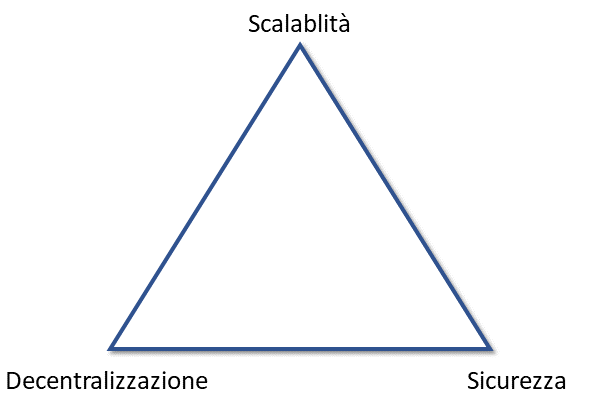
\includegraphics[width=0.6\textwidth]{immagini/trilemmascalab.png}
\caption{Trilemma Scalability}
\label{fig:TrilemmaScalab}
\end{figure}

La combinazione delle proprietà individuate: la decentralizzazione, la scalabilità e la sicurezza, della figura \ref{fig:TrilemmaScalab} prende il nome di \emph{trilemma scalability} \footfullcite{trilemmaScalab}. La difficoltà di mantenere un equilibrio, un compromesso tra queste tre proprietà è uno dei problemi principali del paradigma blockchain. Attualmente è in corso la ricerca sui metodi e sulle soluzioni per ovviare alla necessità di sacrificare almeno una di queste tre proprietà. Un’analisi più approfondita esula dallo scopo di questa tesi, ma è opportuno menzionare un certo numero di direzioni verso quali, al momento dello scrivere, tende la ricerca. Tra questo è lecito considerare come più promettenti le seguenti soluzioni: \emph{sharding}, \emph{sidechains}, \emph{plasma} e molte altre.

Infine per certe applicazioni il trilemma scalability potrebbe non costituire affatto un problema. Nella prossima sezione si parlerà dell’adozione di una tipologia di blockchain con permessi (\emph{permissioned}) che, per ragioni pratiche, non necessitano l’applicazione simultanea delle tre proprietà appena descritte.

\section{Tipologie di un sistema distribuito} %  Inizio sezione 2.4

In funzione dei principi che concorrono alla formazione delle blockchain è ragionevole pensare che, a seconda delle applicazioni che vogliono raggiungere degli obiettivi concreti, sia importante trovare un compromesso tra i vantaggi e gli svantaggi inerenti al paradigma in questione. Infatti è possibile scegliere tra i concetti (descritti nel capitolo 2) per creare un sistema blockchain adatto alle proprie esigenze. Per questo scopo è possibile estrapolare quattro caratteristiche principali del paradigma blockchain:

\begin{itemize}
\item Decentralizzazione
\item Trasparenza
\item Immutabilità
\item Permanenza
\end{itemize}

Insieme questi concetti concorrono alla sicurezza dell'intera rete ma, come è stato già detto, ne derivano problemi relativi a scalability trilemma. Rinunciando a delle proprietà è possibile creare dei sistemi più efficienti, ma che si avvicinano di più ai sistemi informatici attualmente in uso. Pertanto è importante considerare attentamente i requisti del progetto a cui si vorrebbe applicare questa tecnologia per poter valutare in maniera ottimale i vantaggi e gli svantaggi, rispetto ai tradizionali sistemi centralizzati.

\subsection{Unpermissioned Ledgers}

Le blockchain pubbliche o senza permessi sono la tipologia che implementa tutti i concetti descritti fino a questo punto. Sono aperte, non hanno un proprietario e consentono indistintamente a tutti di contribuire e interagire con le risorse della rete. Come affermato in precedenza permettono a tutti di entrare in possesso di un’identica copia del  registro distribuito e universalmente validato dagli utenti della blockchain.

Questa tipologia di blockchain costituisce l’oggetto principale di questa tesi, è il paradigma che ha come presupposto la decentralizzazione del potere e dei dati, rendendo quasi impossibili eventuali tentativi di censura\footfullcite{censorship}. Gli esempi di implementazioni blockchain: Bitcoin ed Ethereum sono delle blockchain pubbliche. È una tipologia promettente ma sulla quale sono necessari altri miglioramenti, in particolare nel settore della scalabilità. In questo modo potrebbero costituire una valida alternativa ai sistemi attuali e competere in un numero di ambiti applicativi maggiore.

\subsection{Permissioned Ledgers}

Le blockchain con permessi (\emph{permissioned}) ammettono di essere più strettamente controllate. Solitamente incorporano un’entità centrale con il compito di gestire le regole della rete, stabilire i permessi degli utenti, la visibilità dei dati e così via, proprio come avviene nei sistemi centralizzati. A seconda delle necessità, in una blockchain di questo tipo, si potrebbe rinunciare a una parte del potere centralizzato o viceversa a una parte delle caratteristiche delle blockchain pubbliche, per creare applicazioni che meglio si adattano alle necessità di enti, imprese e istituzioni interessate. Ad esempio tra le tante possibilità il sistema di consenso potrebbe essere controllato da utenti imposti a priori dal proprietario/i della rete, perché ritenuti fidati. Un'altra opzione utile è relativa ai diritti di leggere o di interagire con i registri, questi permessi potrebbero essere assegnati a certe categorie di utenti. La conseguenza di questo modello è collegata alla diminuzione della decentralizzazione e della trasparenza rispetto alla tipologia senza permessi.

In questo modo è possibile usufruire di alcuni concetti delle blockchain, come la struttura basata sulla crittografia, l’implementazione di smart contracts ecc. allo stesso tempo favorendo la scalabilità della rete stessa. Un esempio rilevante, già accennato in precedenza, riguarda Ripple e il suo sistema di pagamenti fondato sulla blockchain con permessi che, riesce a raggiungere un throughput simile a quello del sistema Visa. Analizzando il funzionamento di attuali sistemi bancari è facile pensare a come le transazioni, in particolare tra banche e nazioni diverse, richiedano tempo e costi connessi alle commissioni. Una potenziale applicazione di \emph{permissioned blockchain}, come Ripple\footfullcite{rippleProtocol}, potrebbe favorire la creazione di standard internazionali con un incremento della velocità di trasferimenti e la relativa diminuzione di costi di mantenimento dovuta ai dati sparsi nei diversi registri bancari.

\section{Blockchain negli archivi digitali} %  Inizio sezione 2.5
\label{sectionDigitalArchives}

Tra i tanti settori interessati alle applicazioni della tecnologia blockchain l’area relativa ai beni culturali e archivi digitali sembra particolarmente promettente. I vantaggi derivati dalla digitalizzazione dei dati in un contesto distribuito potrebbero fornire la risposta ai problemi presenti nelle attuali basi di dati.

Questa sezione si ricollega direttamente al progetto svolto per questa tesi, i cui requisiti dettagliati sono esposti nel capitolo 4.1. Il progetto svolto ha come obiettivo l’inserimento, la consultazione e la verifica di opere d’arte minori. Si vuole dimostrare che i concetti presentati fino a questo punto si prestano bene all'analisi nell’ambito applicativo in questione.

Innanzitutto intuitivamente è possibile dare una prima definizione delle opere d’arte minori: cioè opere meno famose e per qualsiasi motivo giudicate meno importanti dei capolavori artistici. Questo ovviamente non diminuisce la loro importanza a livello culturale e del patrimonio umano, specie in un contesto locale. Anzi, la loro salvaguardia e valorizzazione potrebbero sotto certi aspetti rivelarsi più difficili dei loro corrispettivi “famosi”. Questo perché, spesso questi oggetti sono più vulnerabili ai furti e alle contraffazioni. Una prima azione prioritaria consisterebbe proprio nella registrazione di questi oggetti in un sistema blockchain.

Tenendo in considerazione lo stato dell'arte degli archivi digitali generalmente controllati da un ente centrale con il compito di mantenere e aggiornare il relativo database, è possibile analizzare caratteristiche potenzialmente innovative del paradigma blockchain e il loro impatto in rapporto ai loro corrispettivi tradizionali:

\begin{itemize}
\item La decentralizzazione permette di fare a meno del controllo centrale trasferendo il compito di gestione dell’archivio alla comunità. Riguardo alla disponibilità e al mantenimento di questi sistemi a lungo termine si toglie la responsabilità dei rischi connessi alle attività di organi centrali (ad esempio: cambiamenti di proprietà, mancanza di fondi, gestione di della sicurezza del sistema ecc.), garantendo il possesso di una copia dell’archivio a tutti gli utenti. 
\item Grazie alla permanenza dei dati situati in registri immutabili è possibile garantire la disponibilità degli oggetti digitalizzati a chiunque e in qualunque periodo di tempo. 
\item La trasparenza della rete blockchain favorisce una completa tracciabilità delle opere e i relativi aggiornamenti del loro stato, come i trasferimenti di proprietà e gli spostamenti degli oggetti in questione.
\item L'immutabilità applicata attraverso regole di crittografia contribuisce all’integrità e alla sicurezza del sistema prevenendo fenomeni, come modifiche non autorizzate e tentativi di cancellazione dei dati.
\end{itemize}

Questo breve elenco può risultare utile come punto di partenza per una riflessione finalizzata al miglioramento di sistemi esistenti.